
%% bare_conf.tex
%% V1.4b
%% 2015/08/26
%% by Michael Shell
%% See:
%% http://www.michaelshell.org/
%% for current contact information.
%%
%% This is a skeleton file demonstrating the use of IEEEtran.cls
%% (requires IEEEtran.cls version 1.8b or later) with an IEEE
%% conference paper.
%%alright
%% Support sites:
%% http://www.michaelshell.org/tex/ieeetran/
%% http://www.ctan.org/pkg/ieeetran
%% and
%% http://www.ieee.org/

%%*************************************************************************
%% Legal Notice:
%% This code is offered as-is without any warranty either expressed or
%% implied; without even the implied warranty of MERCHANTABILITY or
%% FITNESS FOR A PARTICULAR PURPOSE! 
%% User assumes all risk.
%% In no event shall the IEEE or any contributor to this code be liable for
%% any damages or losses, including, but not limited to, incidental,
%% consequential, or any other damages, resulting from the use or misuse
%% of any information contained here.
%%
%% All comments are the opinions of their respective authors and are not
%% necessarily endorsed by the IEEE.
%%
%% This work is distributed under the LaTeX Project Public License (LPPL)
%% ( http://www.latex-project.org/ ) version 1.3, and may be freely used,
%% distributed and modified. A copy of the LPPL, version 1.3, is included
%% in the base LaTeX documentation of all distributions of LaTeX released
%% 2003/12/01 or later.
%% Retain all contribution notices and credits.
%% ** Modified files should be clearly indicated as such, including  **
%% ** renaming them and changing author support contact information. **
%%*************************************************************************


% *** Authors should verify (and, if needed, correct) their LaTeX system  ***
% *** with the testflow diagnostic prior to trusting their LaTeX platform ***
% *** with production work. The IEEE's font choices and paper sizes can   ***
% *** trigger bugs that do not appear when using other class files.       ***                          ***
% The testflow support page is at:
% http://www.michaelshell.org/tex/testflow/



\documentclass[conference]{IEEEtran}
% Some Computer Society conferences also require the compsoc mode option,
% but others use the standard conference format.
%
% If IEEEtran.cls has not been installed into the LaTeX system files,
% manually specify the path to it like:
% \documentclass[conference]{../sty/IEEEtran}





% Some very useful LaTeX packages include:
% (uncomment the ones you want to load)


% *** MISC UTILITY PACKAGES ***
%
%\usepackage{ifpdf}
% Heiko Oberdiek's ifpdf.sty is very useful if you need conditional
% compilation based on whether the output is pdf or dvi.
% usage:
% \ifpdf
%   % pdf code
% \else
%   % dvi code
% \fi
% The latest version of ifpdf.sty can be obtained from:
% http://www.ctan.org/pkg/ifpdf
% Also, note that IEEEtran.cls V1.7 and later provides a builtin
% \ifCLASSINFOpdf conditional that works the same way.
% When switching from latex to pdflatex and vice-versa, the compiler may
% have to be run twice to clear warning/error messages.






% *** CITATION PACKAGES ***
%
%\usepackage{cite}
% cite.sty was written by Donald Arseneau
% V1.6 and later of IEEEtran pre-defines the format of the cite.sty package
% \cite{} output to follow that of the IEEE. Loading the cite package will
% result in citation numbers being automatically sorted and properly
% "compressed/ranged". e.g., [1], [9], [2], [7], [5], [6] without using
% cite.sty will become [1], [2], [5]--[7], [9] using cite.sty. cite.sty's
% \cite will automatically add leading space, if needed. Use cite.sty's
% noadjust option (cite.sty V3.8 and later) if you want to turn this off
% such as if a citation ever needs to be enclosed in parenthesis.
% cite.sty is already installed on most LaTeX systems. Be sure and use
% version 5.0 (2009-03-20) and later if using hyperref.sty.
% The latest version can be obtained at:
% http://www.ctan.org/pkg/cite
% The documentation is contained in the cite.sty file itself.






% *** GRAPHICS RELATED PACKAGES ***
%
\ifCLASSINFOpdf
  % \usepackage[pdftex]{graphicx}
  % declare the path(s) where your graphic files are
  % \graphicspath{{../pdf/}{../jpeg/}}
  % and their extensions so you won't have to specify these with
  % every instance of \includegraphics
  % \DeclareGraphicsExtensions{.pdf,.jpeg,.png}
\else
  % or other class option (dvipsone, dvipdf, if not using dvips). graphicx
  % will default to the driver specified in the system graphics.cfg if no
  % driver is specified.
  % \usepackage[dvips]{graphicx}
  % declare the path(s) where your graphic files are
  % \graphicspath{{../eps/}}
  % and their extensions so you won't have to specify these with
  % every instance of \includegraphics
  % \DeclareGraphicsExtensions{.eps}
\fi
% graphicx was written by David Carlisle and Sebastian Rahtz. It is
% required if you want graphics, photos, etc. graphicx.sty is already
% installed on most LaTeX systems. The latest version and documentation
% can be obtained at: 
% http://www.ctan.org/pkg/graphicx
% Another good source of documentation is "Using Imported Graphics in
% LaTeX2e" by Keith Reckdahl which can be found at:
% http://www.ctan.org/pkg/epslatex
%
% latex, and pdflatex in dvi mode, support graphics in encapsulated
% postscript (.eps) format. pdflatex in pdf mode supports graphics
% in .pdf, .jpeg, .png and .mps (metapost) formats. Users should ensure
% that all non-photo figures use a vector format (.eps, .pdf, .mps) and
% not a bitmapped formats (.jpeg, .png). The IEEE frowns on bitmapped formats
% which can result in "jaggedy"/blurry rendering of lines and letters as
% well as large increases in file sizes.
%
% You can find documentation about the pdfTeX application at:
% http://www.tug.org/applications/pdftex





% *** MATH PACKAGES ***
%
%\usepackage{amsmath}
% A popular package from the American Mathematical Society that provides
% many useful and powerful commands for dealing with mathematics.
%
% Note that the amsmath package sets \interdisplaylinepenalty to 10000
% thus preventing page breaks from occurring within multiline equations. Use:
%\interdisplaylinepenalty=2500
% after loading amsmath to restore such page breaks as IEEEtran.cls normally
% does. amsmath.sty is already installed on most LaTeX systems. The latest
% version and documentation can be obtained at:
% http://www.ctan.org/pkg/amsmath





% *** SPECIALIZED LIST PACKAGES ***
%
%\usepackage{algorithmic}
% algorithmic.sty was written by Peter Williams and Rogerio Brito.
% This package provides an algorithmic environment fo describing algorithms.
% You can use the algorithmic environment in-text or within a figure
% environment to provide for a floating algorithm. Do NOT use the algorithm
% floating environment provided by algorithm.sty (by the same authors) or
% algorithm2e.sty (by Christophe Fiorio) as the IEEE does not use dedicated
% algorithm float types and packages that provide these will not provide
% correct IEEE style captions. The latest version and documentation of
% algorithmic.sty can be obtained at:
% http://www.ctan.org/pkg/algorithms
% Also of interest may be the (relatively newer and more customizable)
% algorithmicx.sty package by Szasz Janos:
% http://www.ctan.org/pkg/algorithmicx




% *** ALIGNMENT PACKAGES ***
%
%\usepackage{array}
% Frank Mittelbach's and David Carlisle's array.sty patches and improves
% the standard LaTeX2e array and tabular environments to provide better
% appearance and additional user controls. As the default LaTeX2e table
% generation code is lacking to the point of almost being broken with
% respect to the quality of the end results, all users are strongly
% advised to use an enhanced (at the very least that provided by array.sty)
% set of table tools. array.sty is already installed on most systems. The
% latest version and documentation can be obtained at:
% http://www.ctan.org/pkg/array


% IEEEtran contains the IEEEeqnarray family of commands that can be used to
% generate multiline equations as well as matrices, tables, etc., of high
% quality.




% *** SUBFIGURE PACKAGES ***
%\ifCLASSOPTIONcompsoc
%  \usepackage[caption=false,font=normalsize,labelfont=sf,textfont=sf]{subfig}
%\else
%  \usepackage[caption=false,font=footnotesize]{subfig}
%\fi
% subfig.sty, written by Steven Douglas Cochran, is the modern replacement
% for subfigure.sty, the latter of which is no longer maintained and is
% incompatible with some LaTeX packages including fixltx2e. However,
% subfig.sty requires and automatically loads Axel Sommerfeldt's caption.sty
% which will override IEEEtran.cls' handling of captions and this will result
% in non-IEEE style figure/table captions. To prevent this problem, be sure
% and invoke subfig.sty's "caption=false" package option (available since
% subfig.sty version 1.3, 2005/06/28) as this is will preserve IEEEtran.cls
% handling of captions.
% Note that the Computer Society format requires a larger sans serif font
% than the serif footnote size font used in traditional IEEE formatting
% and thus the need to invoke different subfig.sty package options depending
% on whether compsoc mode has been enabled.
%
% The latest version and documentation of subfig.sty can be obtained at:
% http://www.ctan.org/pkg/subfig




% *** FLOAT PACKAGES ***
%
%\usepackage{fixltx2e}
% fixltx2e, the successor to the earlier fix2col.sty, was written by
% Frank Mittelbach and David Carlisle. This package corrects a few problems
% in the LaTeX2e kernel, the most notable of which is that in current
% LaTeX2e releases, the ordering of single and double column floats is not
% guaranteed to be preserved. Thus, an unpatched LaTeX2e can allow a
% single column figure to be placed prior to an earlier double column
% figure.
% Be aware that LaTeX2e kernels dated 2015 and later have fixltx2e.sty's
% corrections already built into the system in which case a warning will
% be issued if an attempt is made to load fixltx2e.sty as it is no longer
% needed.
% The latest version and documentation can be found at:
% http://www.ctan.org/pkg/fixltx2e


%\usepackage{stfloats}
% stfloats.sty was written by Sigitas Tolusis. This package gives LaTeX2e
% the ability to do double column floats at the bottom of the page as well
% as the top. (e.g., "\begin{figure*}[!b]" is not normally possible in
% LaTeX2e). It also provides a command:
%\fnbelowfloat
% to enable the placement of footnotes below bottom floats (the standard
% LaTeX2e kernel puts them above bottom floats). This is an invasive package
% which rewrites many portions of the LaTeX2e float routines. It may not work
% with other packages that modify the LaTeX2e float routines. The latest
% version and documentation can be obtained at:
% http://www.ctan.org/pkg/stfloats
% Do not use the stfloats baselinefloat ability as the IEEE does not allow
% \baselineskip to stretch. Authors submitting work to the IEEE should note
% that the IEEE rarely uses double column equations and that authors should try
% to avoid such use. Do not be tempted to use the cuted.sty or midfloat.sty
% packages (also by Sigitas Tolusis) as the IEEE does not format its papers in
% such ways.
% Do not attempt to use stfloats with fixltx2e as they are incompatible.
% Instead, use Morten Hogholm'a dblfloatfix which combines the features
% of both fixltx2e and stfloats:
%
% \usepackage{dblfloatfix}
% The latest version can be found at:
% http://www.ctan.org/pkg/dblfloatfix




% *** PDF, URL AND HYPERLINK PACKAGES ***
%
%\usepackage{url}
% url.sty was written by Donald Arseneau. It provides better support for
% handling and breaking URLs. url.sty is already installed on most LaTeX
% systems. The latest version and documentation can be obtained at:
% http://www.ctan.org/pkg/url
% Basically, \url{my_url_here}.




% *** Do not adjust lengths that control margins, column widths, etc. ***
% *** Do not use packages that alter fonts (such as pslatex).         ***
% There should be no need to do such things with IEEEtran.cls V1.6 and later.
% (Unless specifically asked to do so by the journal or conference you plan
% to submit to, of course. )
\usepackage{pifont}
\usepackage{cite}
\usepackage{caption}
%\usepackage{subcaption}
\usepackage{url}
\usepackage{multirow}
\usepackage[cmex10]{amsmath}
\usepackage{amsmath,amssymb}
%\usepackage{algorithmic}
\usepackage{mdwmath}
\usepackage{float}
\usepackage{amsmath}
\usepackage[T1]{fontenc}
\usepackage{graphicx}
\usepackage{varwidth,xcolor}

%\usepackage[ruled,noresetcount,noend]{algorithm2e}
%\usepackage{algorithm}% http://ctan.org/pkg/algorithms
\usepackage{algpseudocode}
\usepackage{array}
\usepackage{program}
\usepackage{float}
\usepackage[caption = false]{subfig}
\usepackage{algorithm}
\usepackage{algpseudocode}
% correct bad hyphenation here
\hyphenation{op-tical net-works semi-conduc-tor}


\begin{document}
%
% paper title
% Titles are generally capitalized except for words such as a, an, and, as,
% at, but, by, for, in, nor, of, on, or, the, to and up, which are usually
% not capitalized unless they are the first or last word of the title.
% Linebreaks \\ can be used within to get better formatting as desired.
% Do not put math or special symbols in the title.
\title{Travelling Salesman Problem\\ simulated with Simple Genetic Algorithm}


% author names and affiliations
% use a multiple column layout for up to three different
% affiliations
\author{\IEEEauthorblockN{Kevin Tram}
\IEEEauthorblockA{Computer Science\\
Brock University\\
St Catharines, Ontario Canada\\
Student Number: 5459854\\
Email: kt13nh@brocku.ca}}

% conference papers do not typically use \thanks and this command
% is locked out in conference mode. If really needed, such as for
% the acknowledgment of grants, issue a \IEEEoverridecommandlockouts
% after \documentclass

% for over three affiliations, or if they all won't fit within the width
% of the page, use this alternative format:
% 
%\author{\IEEEauthorblockN{Michael Shell\IEEEauthorrefmark{1},
%Homer Simpson\IEEEauthorrefmark{2},
%James Kirk\IEEEauthorrefmark{3}, 
%Montgomery Scott\IEEEauthorrefmark{3} and
%Eldon Tyrell\IEEEauthorrefmark{4}}
%\IEEEauthorblockA{\IEEEauthorrefmark{1}School of Electrical and Computer Engineering\\
%Georgia Institute of Technology,
%Atlanta, Georgia 30332--0250\\ Email: see http://www.michaelshell.org/contact.html}
%\IEEEauthorblockA{\IEEEauthorrefmark{2}Twentieth Century Fox, Springfield, USA\\
%Email: homer@thesimpsons.com}
%\IEEEauthorblockA{\IEEEauthorrefmark{3}Starfleet Academy, San Francisco, California 96678-2391\\
%Telephone: (800) 555--1212, Fax: (888) 555--1212}
%\IEEEauthorblockA{\IEEEauthorrefmark{4}Tyrell Inc., 123 Replicant Street, Los Angeles, California 90210--4321}}




% use for special paper notices
%\IEEEspecialpapernotice{(Invited Paper)}




% make the title area
\maketitle

% As a general rule, do not put math, special symbols or citations
% in the abstract
\begin{abstract}
Travelling salesman problem, a very well known problem among the computer science community, tries the solve this problem with a variety of different strategies and algorithms. The problem is this: if a salesman must visit all the cities in a given place, what is a good route that the salesman can follow to efficiently travel to visit all of the cities? At first glance, one can imagine with a small data set, it can be relatively easy to determine the shortest path by simple trial and error. However, as we're going to see with "berlin52" and "djibouti38" data set, this is not the case. In this report, we will examine these two data sets and observe the significant impact genetic algorithms can have on the solutions of each of these data sets. Each solution is a representation of a route, where experiments will be conducted in an attempt to solve the TSP problem with a reasonably good solutions with two different crossovers, and one type of mutation. It is observed that Order Crossover generally performed better than Uniform Order Crossover.
\end{abstract}

% no keywords




% For peer review papers, you can put extra information on the cover
% page as needed:
% \ifCLASSOPTIONpeerreview
% \begin{center} \bfseries EDICS Category: 3-BBND \end{center}
% \fi
%
% For peerreview papers, this IEEEtran command inserts a page break and
% creates the second title. It will be ignored for other modes.
\IEEEpeerreviewmaketitle



\section{Introduction}
The Travelling salesman problem was first introduced in 1930 and since, one of the most studied optimization problems by scholars. This is an NP-Hard problem used as a benchmark for many different optimization methods, genetic algorithms included. The experiment will look at how different genetic algorithms including a variety of crossover methods, mutations, and parameters will affect the outcome best route distances of every generation. These different methods of crossover and parameters will be compared against each other in terms of performance, examined to determine which will yield the best possible solutions for each of the datasets provided. 

\subsection{Objective and problem definition}
With the provided data sets "Berlin52", and "Djibouti38" a possible good solution is found by implementing a simple genetic algorithm incorporating a variety of different user parameters for crossover rates, mutation rates, and types of crossovers. This main problem is defined as: a salesman must travel to all of the cities in a specific area at least once. This problem represented based on genetic algorithms using chromosome solutions as cities, as well as always ensuring the chromosomes are valid tsp solutions. Each chromosome is represented as a set of genes, and each gene is represented as a city, where each collection of genes is representation for a valid solution. Every city contains relevant attributes, such as its X-coordinate, and Y-coordinate. Distance among city to city is calculated using the well known Euclidean distance illustrated below: 


\subsubsection{Euclidean Distance Equation}
\begin{equation}
	d=\sqrt{((x_1-x_2)^2 + (y_1-y_2)^2)}
\end{equation}

After new generation productions, the hope is to develop parent solutions into better solutions using an elite strategy where the best chromosome from the previous generation is always going to be included in the next generation. We will analyze the solutions being produced by the simple genetic algorithm with Uniform Order Crossover and Order Crossover. Inversion mutation will also have a chance to be applied to each of the genes in the next generation as entered by the parameters. Tournament selection will be used for all of the new generations where k-value 3 is used to determine which chromosome is to make it through the tournament. Once selection is complete, crossover and mutations are applied to the new offspring. After producing many generations, and inheriting the best chromosome after every generation, the difference in fitness of the chromosomes produced in the genetic algorithm will be observed, and used determine the best user parameter settings, with crossover and mutation rates. This will be achieved with the following simple GA algorithm:

\begin{algorithm}
\caption{Simple GA:}
\label{GA}
\begin{algorithmic}[1]
\Procedure{Simple GA}{}
	\State $Begin$
	\State $Read $ $problem $ $instance $ $data;$
	\State $Generate $ $random $ $initial $ $POP $ $of  $ $size $ $PopSize;$
    \For {gen = 1 to MAXGEN}
        \State $Evaluate $ $fitness $ $of $ 			$the $ $individuals $ $of $ $POP;$
        \State $Select $ $new $ $POP $ $using $ $tournament $ $selection;$
        \State $Apply $ $genetic $ 						$operators, $ $crossover,$				$mutation;$
	\EndFor
	\State $end;$
\EndProcedure
\end{algorithmic}
\end{algorithm}

\subsection{Summary Parameters Used}
\subsubsection{Berlin52 Uniform Order Crossover}


The following parameters are used in the experiment of Berlin52 using Uniform order Crossover and Inversion Mutation:
\graphicspath{ {Parameter_results/} }
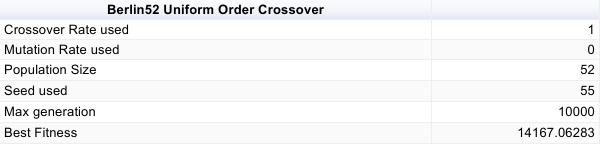
\includegraphics[scale=0.42]{Berlin52/UOC/Berlin52_UOC_a)_table}
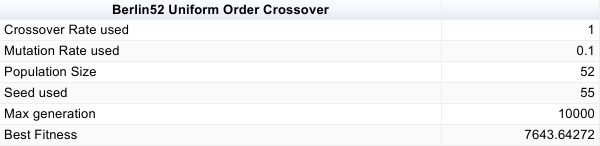
\includegraphics[scale=0.42]{Berlin52/UOC/Berlin52_UOC_b)_table}
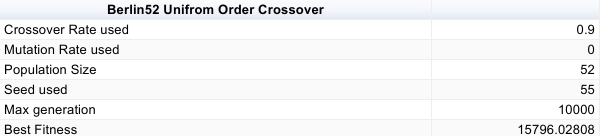
\includegraphics[scale=0.42]{Berlin52/UOC/Berlin52_UOC_c)_table}
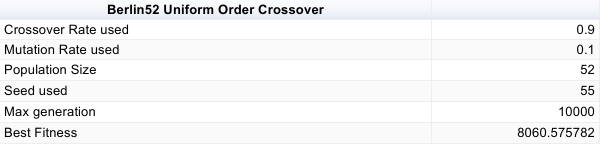
\includegraphics[scale=0.42]{Berlin52/UOC/Berlin52_UOC_d)_table}
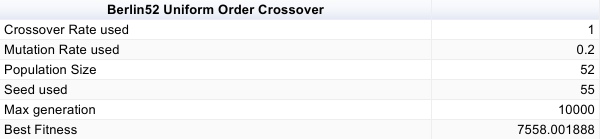
\includegraphics[scale=0.42]{Berlin52/UOC/Berlin52_UOC_e)_table}

As easily observed in the above parameter selections, the crossover rate of 1 and mutation rate of 0.2 yielded the most efficient solution for the Berlin52 dataset using Uniform Order Crossover and maximum generation 10,000.

\subsubsection{Berlin52 Order Crossover}

The following parameters are used in the experiment of Berlin52 using Order Crossover and Inversion Mutation:
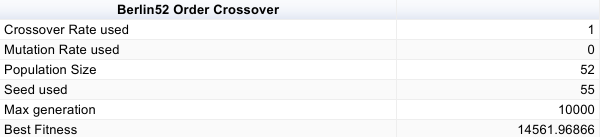
\includegraphics[scale=0.42]{Berlin52/OC/Berlin52_OC_a)_table}
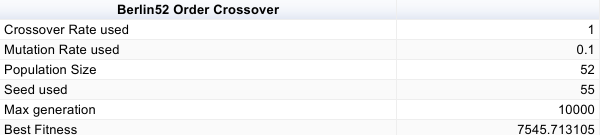
\includegraphics[scale=0.42]{Berlin52/OC/Berlin52_OC_b)_table}
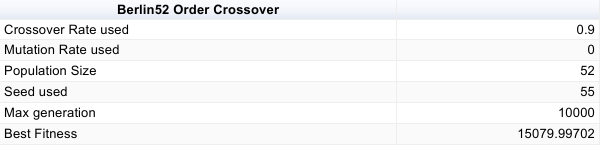
\includegraphics[scale=0.42]{Berlin52/OC/Berlin52_OC_c)_table}
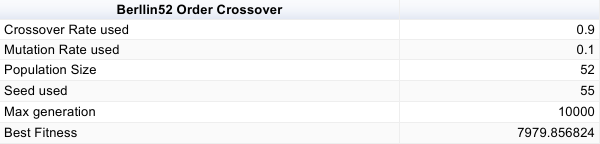
\includegraphics[scale=0.42]{Berlin52/OC/Berlin52_OC_d)_table}
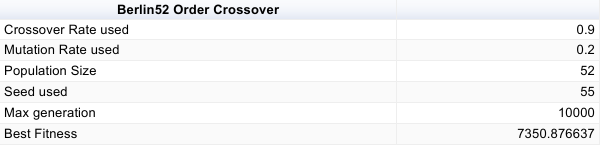
\includegraphics[scale=0.42]{Berlin52/OC/Berlin52_OC_e)_table}


As observed in the above tables of Order Crossover experimented with the Berlin52 dataset, crossover rate of 0.9 and mutation rate of 0.2 yielded the most optimal fitness value with maximum generation 10,000.

\subsubsection{Djibouti38 Uniform Order Crossover}

The following parameters are used in the experiment of Djibouti38 using Uniform Order Crossover and Inversion Mutation:
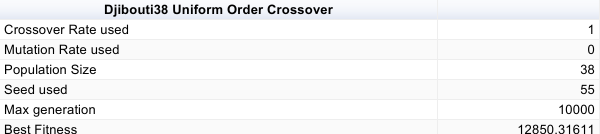
\includegraphics[scale=0.42]{Djibouti38/UOC/Djibouti38_UOC_a)_table}
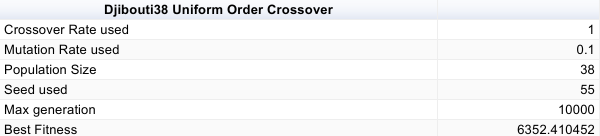
\includegraphics[scale=0.42]{Djibouti38/UOC/Djibouti38_UOC_b)_table}
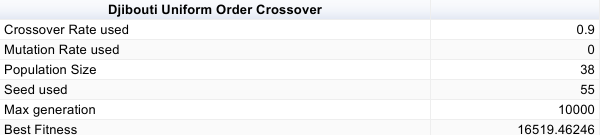
\includegraphics[scale=0.42]{Djibouti38/UOC/Djibouti38_UOC_c)_table}
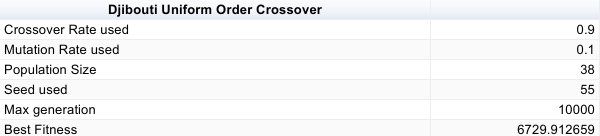
\includegraphics[scale=0.42]{Djibouti38/UOC/Djibouti38_UOC_d)_table}
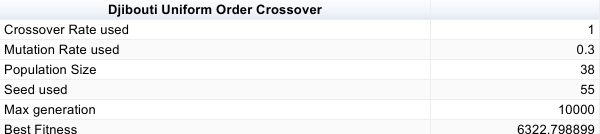
\includegraphics[scale=0.42]{Djibouti38/UOC/Djibouti38_UOC_e)_table}

As observed in the above tables of Uniform Order Crossover experimented with the dataset Djibouti38, a crossover rate of 1 and mutation rate of 0.3 yielded the most optimal fitness value with maximum generation 10,000. 

\subsubsection{Djibouti38 Order Crossover}

The following parameters are used in the experiment of Djibouti38 using Uniform Order Crossover and Inversion Mutation:
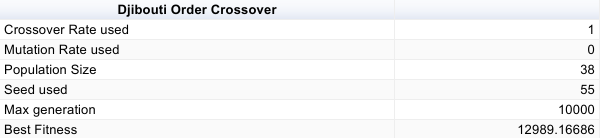
\includegraphics[scale=0.42]{Djibouti38/OC/Djibouti38_OC_a)_table}
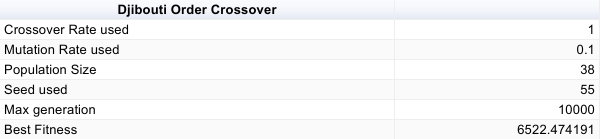
\includegraphics[scale=0.42]{Djibouti38/OC/Djibouti38_OC_b)_table}
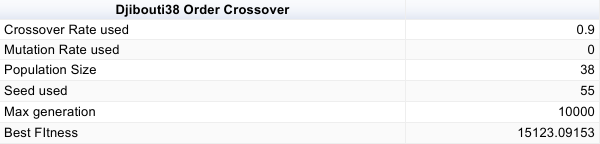
\includegraphics[scale=0.42]{Djibouti38/OC/Djibouti38_OC_c)_table}
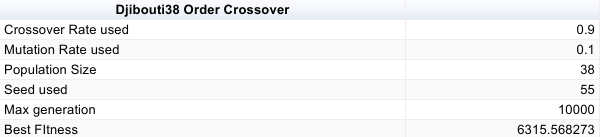
\includegraphics[scale=0.42]{Djibouti38/OC/Djibouti38_OC_d)_table}
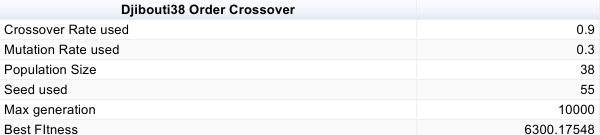
\includegraphics[scale=0.42]{Djibouti38/OC/Djibouti38_OC_e)_table}

As observed in the above tables of Order Crossover experimented with the dataset Djibouti38 a crossover rate of 0.9 and mutation rate of 0.3 yield the most efficient chromosome fitness value with maximum generation of 10,000.

All of the user parameters used are consistent throughout all of the simulation data. Population size of the number of cities are used, as well as a seed of 55 and max generation are kept consistent among all of the simulations in an attempt to gather data to compare uniform order crossover with order crossover.

\subsection{Results}

Berlin52 Uniform Order Crossover a)
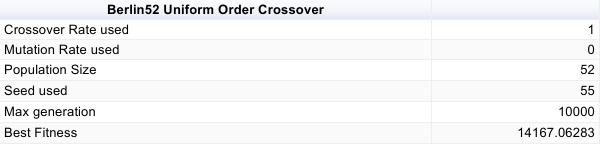
\includegraphics[scale=0.42]{Berlin52/UOC/Berlin52_UOC_a)_table}
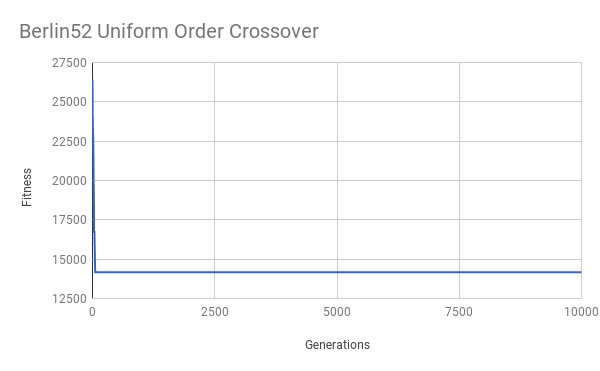
\includegraphics[scale=0.42]{Berlin52/UOC/Berlin52_UOC_a)}
From the above graph an the drastic slope in the beginning generations improves in fitness significantly. However, shortly after the earlier generations the fitness completely plateaus, indicating the limitations of a GA without mutation. It seems as though all of the chromosomes after the initial improvements in fitness suffer from farther improvements due to the lack of diversity in the population. Overall, these parameters have proven to not be useful in terms of evolving for better offspring.

Berlin52 Uniform Order Crossover b)
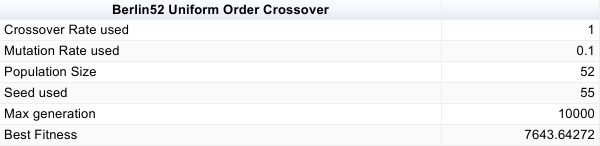
\includegraphics[scale=0.42]{Berlin52/UOC/Berlin52_UOC_b)_table}
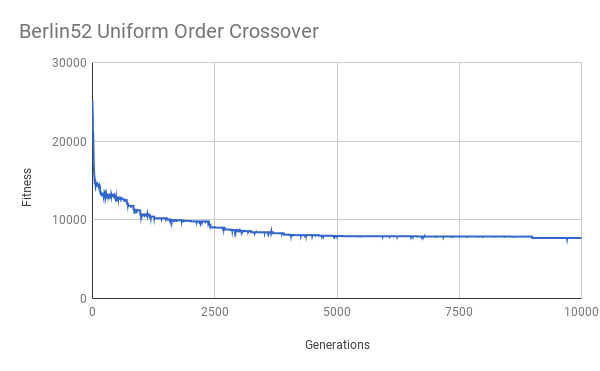
\includegraphics[scale=0.42]{Berlin52/UOC/Berlin52_UOC_b)}
The above graph with the specified parameters improved drastically in fitness from the early generations. They plateau slightly on the 5000 generations mark, however, fitness seems to improve as more generations are improved. A much improvement over graph a), where fitness improve greatly from increasing mutation rate to 0.1. This may indicate slight mutations in each generation will improve the chromosome offspring.

Berlin52 Uniform Order Crossover c)
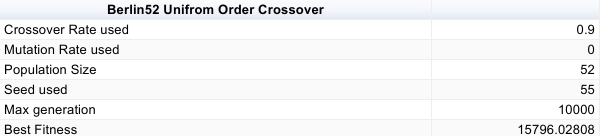
\includegraphics[scale=0.42]{Berlin52/UOC/Berlin52_UOC_c)_table}
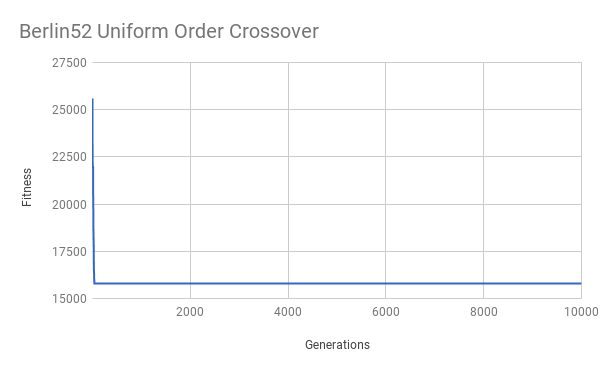
\includegraphics[scale=0.42]{Berlin52/UOC/Berlin52_UOC_c)}
The above graph is much like graph a). There is a sheer improvement in the early generations, but plateaus quickly in a rather inefficient solution after 10,000 generations. With a best fitness value of less than graph a), this may also indicate chromosomes benefit from crossover where offspring will include the good parts of the parent chromosomes and carry forward to spawn even better offspring. These parameters have proven to be inefficient.\\

Berlin52 Uniform Order Crossover d)
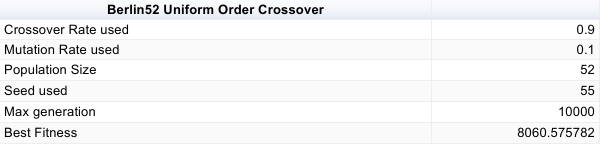
\includegraphics[scale=0.42]{Berlin52/UOC/Berlin52_UOC_d)_table}
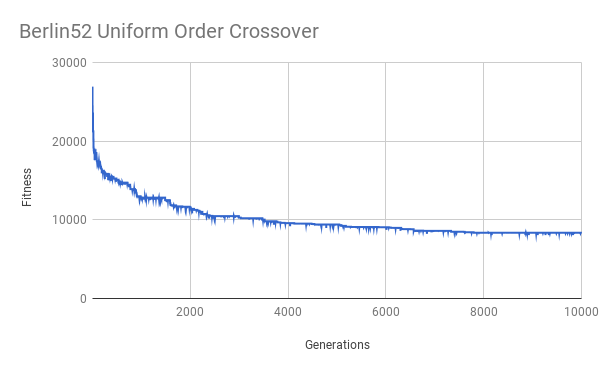
\includegraphics[scale=0.42]{Berlin52/UOC/Berlin52_UOC_d)}
The above graph shows constant signs of improvement, however, still not yielding fitness values as efficient as graph b). Since the crossover rate is less than b), there can be an assumption that higher crossover rates are beneficial to create more efficient children chromosomes than the parents, similar to the evidence presented from graph c).\\

Berlin52 Uniform Order Crossover e)
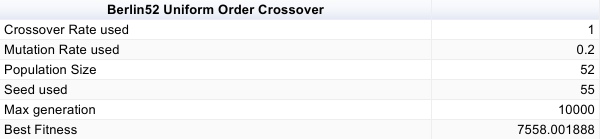
\includegraphics[scale=0.42]{Berlin52/UOC/Berlin52_UOC_e)_table}
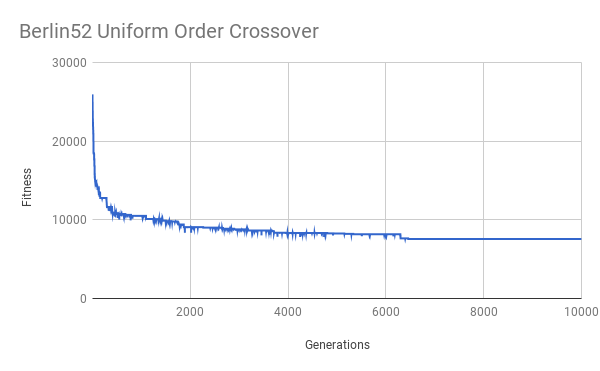
\includegraphics[scale=0.42]{Berlin52/UOC/Berlin52_UOC_e)}
From the evidence observed from graphs a) to d), a crossover rate of 1, and mutation rate of 0.2 is simulated based on the assumptions that high crossover rates are beneficial, as well as some mutations. The resulting fitness is an improvement over all of the Berlin52 Uniform Order Crossover graphs, and thus, the observations regarding chromosome fitness based on crossover rates and mutations are true.\\

Berlin52 Order Crossover a)
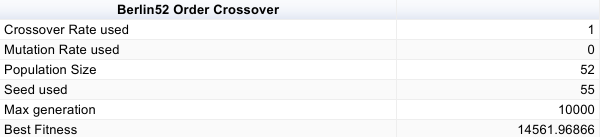
\includegraphics[scale=0.42]{Berlin52/OC/Berlin52_OC_a)_table}
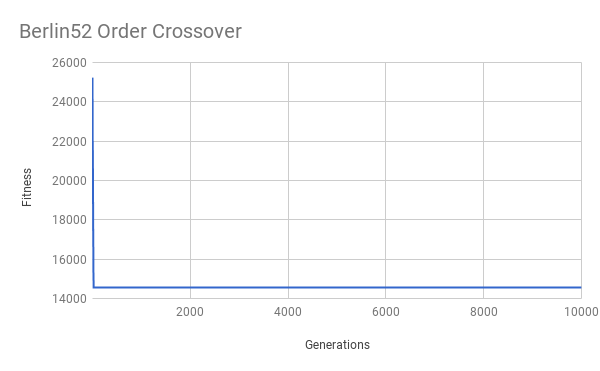
\includegraphics[scale=0.42]{Berlin52/OC/Berlin52_OC_a)}
There is a clear observation this set of parameters show very limited signs of improved chromosomes, and quick plateau that never improves. This is an obvious indicator this set will produce inefficient chromosomes as see by the plateau and the observed best fitness.\\

Berlin52 Order Crossover b)
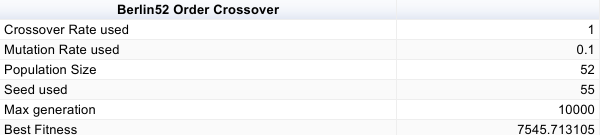
\includegraphics[scale=0.42]{Berlin52/OC/Berlin52_OC_b)_table}
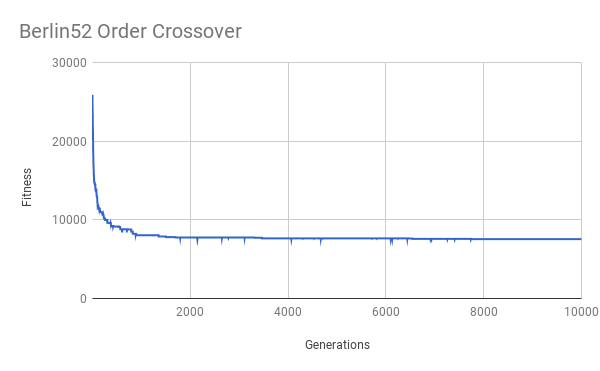
\includegraphics[scale=0.42]{Berlin52/OC/Berlin52_OC_b)}
As soon as mutation rate is increased from graph a), there is an immediate improve in performance. This is further indication that some mutations may yield increase of GA performance. Although plateau is evident past the 8000 generation mark, previous to that there are slight increases in performance throughout the generations.\\


Berlin52 Order Crossover c)
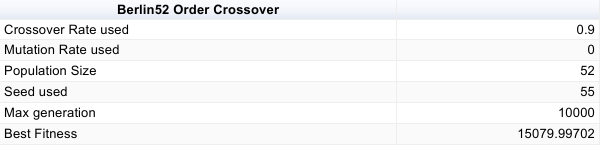
\includegraphics[scale=0.42]{Berlin52/OC/Berlin52_OC_c)_table}
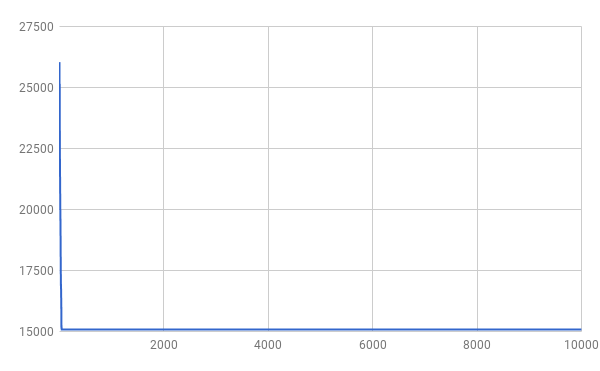
\includegraphics[scale=0.42]{Berlin52/OC/Berlin52_OC_c)}
The above graph is observed with less crossover rate than graph a), and with the same mutation rate, indicating that higher crossover rates will produce better offspring chromosomes. The sheer improvement in the early generations quickly plateau with no signs of improvement and a yield of a very low fitness value proves this set of parameters is inefficient. \\



Berlin52 Order Crossover d)
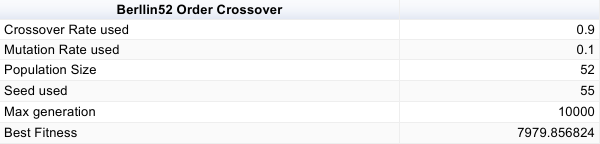
\includegraphics[scale=0.42]{Berlin52/OC/Berlin52_OC_d)_table}
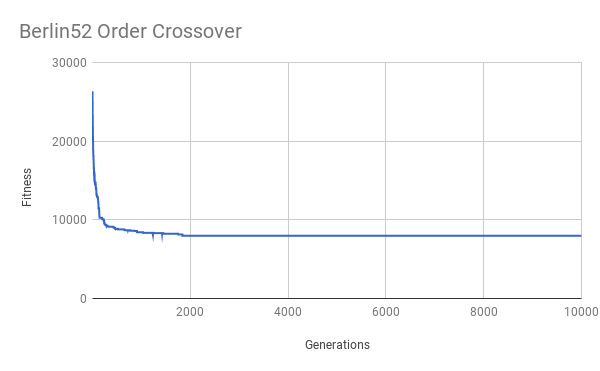
\includegraphics[scale=0.42]{Berlin52/OC/Berlin52_OC_d)}
The above graph with the same parameters as graph c), except for added mutation is a great increase in performance. Although plateaus, the offspring are close to 2 times better fitness than those of c). \\


Berlin52 Order Crossover e)
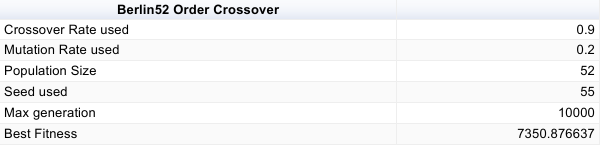
\includegraphics[scale=0.42]{Berlin52/OC/Berlin52_OC_e)_table}
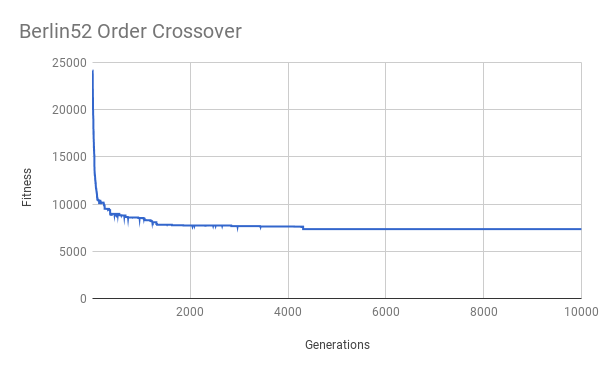
\includegraphics[scale=0.42]{Berlin52/OC/Berlin52_OC_e)}
With the observations from the Order Crossover, the parameters of crossover rate 0.9, and mutation rate of 0.2 is experimented. The Best fitness chromosome yielded better results than all of the observed Berlin52 graphs. Although tested with a 0.9 crossover, this may be indication Order Crossover is more efficient than Uniform Order Crossover on the dataset Berlin52.\\


Djibouti38 Uniform Order Crossover a)
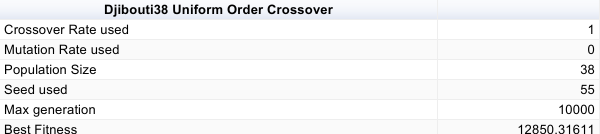
\includegraphics[scale=0.42]{Djibouti38/UOC/Djibouti38_UOC_a)_table}
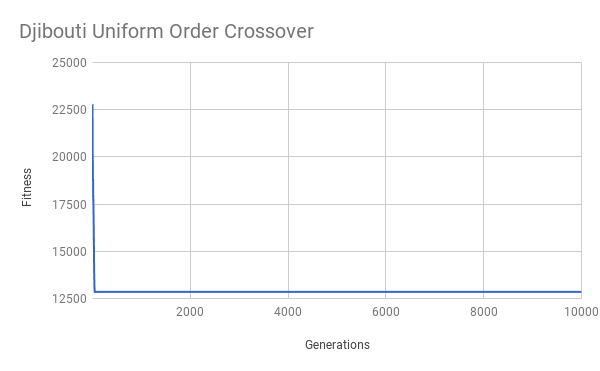
\includegraphics[scale=0.42]{Djibouti38/UOC/Djibouti38_UOC_a)}
The above graph is consistent with the same parameters observed in the Berlin52 data set. There is a drastic improvement in fitness only to plateau quick and never improve again, yielding a very inefficient solution.\\


Djibouti38 Uniform Order Crossover b)
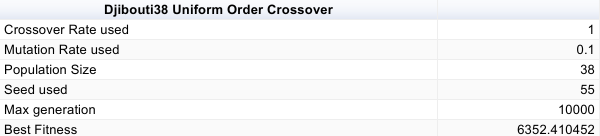
\includegraphics[scale=0.42]{Djibouti38/UOC/Djibouti38_UOC_b)_table}
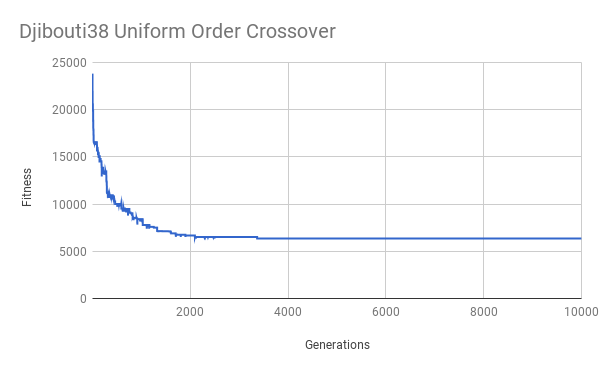
\includegraphics[scale=0.42]{Djibouti38/UOC/Djibouti38_UOC_b)}
The mutation added, the graph is also consistent with the same parameters observed in Berlin52 where the graph will continually improve for several thousand generations until a plateau. This is yielding a good chromosome, though it seems to not improve after the plateau.\\


Djibouti38 Uniform Order Crossover c)
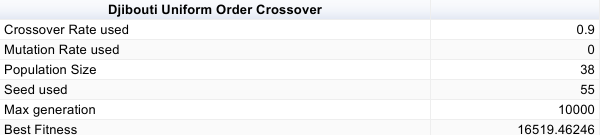
\includegraphics[scale=0.42]{Djibouti38/UOC/Djibouti38_UOC_c)_table}
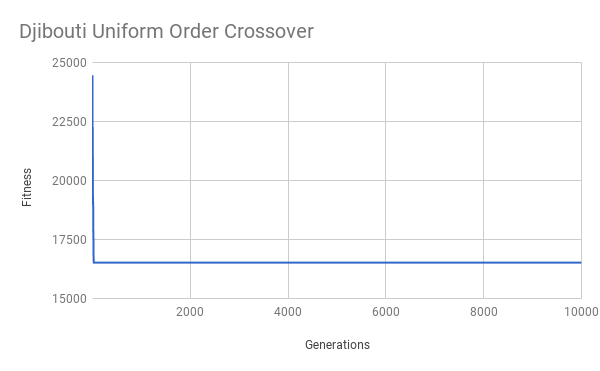
\includegraphics[scale=0.42]{Djibouti38/UOC/Djibouti38_UOC_c)}
Much like graph a), this above graph yield an even worst solution with drastic beginning generation improvements, only to never improve again.\\


Djibouti38 Uniform Order Crossover d)
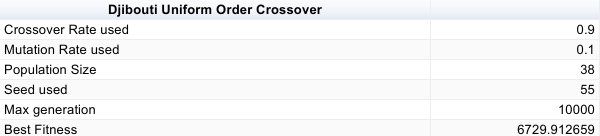
\includegraphics[scale=0.42]{Djibouti38/UOC/Djibouti38_UOC_d)_table}
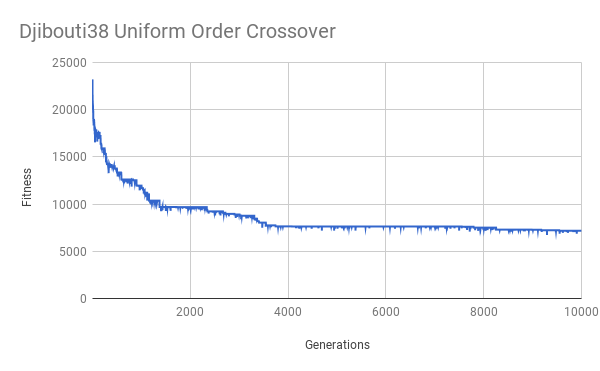
\includegraphics[scale=0.42]{Djibouti38/UOC/Djibouti38_UOC_d)}
The graph above shows constant improvements in fitness, indicating the production of better offspring don't stop since it is observed the graph is jagged towards 10,000th generation, but showing no signs of complete plateau. Although this does not yield a better solution than graph b), graph b) is observed to plateau not not improve offspring again, with graph d) constantly improving chromosomes.\\


Djibouti38 Uniform Order Crossover e)
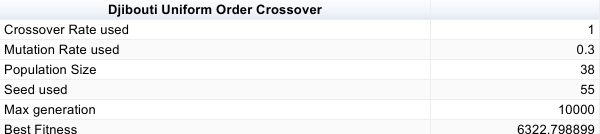
\includegraphics[scale=0.42]{Djibouti38/UOC/Djibouti38_UOC_e)_table}
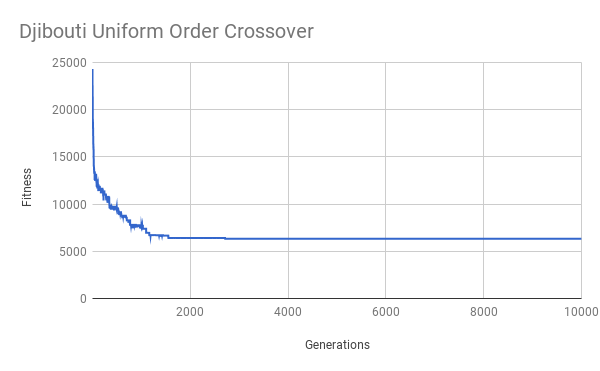
\includegraphics[scale=0.42]{Djibouti38/UOC/Djibouti38_UOC_e)}
From all of the previous observations, an experiment was conducted on the basis that high crossover rates, and high mutation rate will yield good solutions. The graph seems to improve for over 1000 generations, and plateau after 2000. Although this yield better solutions than the other Djibouti Uniform crossover experiments, the plateau never seems to end and chromosomes never improve.


Djibouti38 Order Crossover a)
\includegraphics[scale=0.42]{Djibouti38/OC/Djibouti38_OC_a)_table}
\includegraphics[scale=0.42]{Djibouti38/OC/Djibouti38_OC_a)}
Drastic early generation improvement, also plateau early to never improve offspring again. This is inefficient as observed in all of the experiments conducted with this parameter setting.\\


Djibouti38 Order Crossover b)
\includegraphics[scale=0.42]{Djibouti38/OC/Djibouti38_OC_b)_table}
\includegraphics[scale=0.42]{Djibouti38/OC/Djibouti38_OC_b)}
Very consistent with the other experiments conducted with the same parameter, it is observed that there is a continual improvement in offspring until slightly after the 2000th generation where it will plateau and offspring will not improve. However, still yielding a good solution.\\


Djibouti38 Order Crossover c)
\includegraphics[scale=0.42]{Djibouti38/OC/Djibouti38_OC_c)_table}
\includegraphics[scale=0.42]{Djibouti38/OC/Djibouti38_OC_c)}
Consistent with all of the other experiments conducted with the same parameters. Yields a very inefficient solution.\\

Djibouti38 Order Crossover d)
\includegraphics[scale=0.42]{Djibouti38/OC/Djibouti38_OC_d)_table}
\includegraphics[scale=0.42]{Djibouti38/OC/Djibouti38_OC_d)}
Yielding a better solution than graph b), this may be indication Order Crossover benefits greater from crossover rates slightly less than 100 percent. Although a better fitness value is observed, a similar effect on the chromosome are observed where there is continual improvements in offspring until the 2000th generation. The plateau occurs and never seems to fluctuate.\\



Djibouti38 Order Crossover e)
\includegraphics[scale=0.42]{Djibouti38/OC/Djibouti38_OC_e)_table}
\includegraphics[scale=0.42]{Djibouti38/OC/Djibouti38_OC_e)}
With the observations made on Djibouti38 dataset experiments on order crossover, an approach of crossover value slightly less than 100 percent is used, with 0.3 mutation rate. This yields a better solution than graph d) with similar effect on the offspring chromosomes plateau. This may be indication order crossover benefits from slightly higher mutation rates and slightly lower crossover rates.
% An example of a floating figure using the graphicx package.
% Note that \label must occur AFTER (or within) \caption.
% For figures, \caption should occur after the \includegraphics.
% Note that IEEEtran v1.7 and later has special internal code that
% is designed to preserve the operation of \label within \caption
% even when the captionsoff option is in effect. However, because
% of issues like this, it may be the safest practice to put all your
% \label just after \caption rather than within \caption{}.
%
% Reminder: the "draftcls" or "draftclsnofoot", not "draft", class
% option should be used if it is desired that the figures are to be
% displayed while in draft mode.
%
%\begin{figure}[!t]
%\centering
%\includegraphics[width=2.5in]{myfigure}
% where an .eps filename suffix will be assumed under latex, 
% and a .pdf suffix will be assumed for pdflatex; or what has been declared
% via \DeclareGraphicsExtensions.
%\caption{Simulation results for the network.}
%\label{fig_sim}
%\end{figure}

% Note that the IEEE typically puts floats only at the top, even when this
% results in a large percentage of a column being occupied by floats.


% An example of a double column floating figure using two subfigures.
% (The subfig.sty package must be loaded for this to work.)
% The subfigure \label commands are set within each subfloat command,
% and the \label for the overall figure must come after \caption.
% \hfil is used as a separator to get equal spacing.
% Watch out that the combined width of all the subfigures on a 
% line do not exceed the text width or a line break will occur.
%
%\begin{figure*}[!t]
%\centering
%\subfloat[Case I]{\includegraphics[width=2.5in]{box}%
%\label{fig_first_case}}
%\hfil
%\subfloat[Case II]{\includegraphics[width=2.5in]{box}%
%\label{fig_second_case}}
%\caption{Simulation results for the network.}
%\label{fig_sim}
%\end{figure*}
%
% Note that often IEEE papers with subfigures do not employ subfigure
% captions (using the optional argument to \subfloat[]), but instead will
% reference/describe all of them (a), (b), etc., within the main caption.
% Be aware that for subfig.sty to generate the (a), (b), etc., subfigure
% labels, the optional argument to \subfloat must be present. If a
% subcaption is not desired, just leave its contents blank,
% e.g., \subfloat[].


% An example of a floating table. Note that, for IEEE style tables, the
% \caption command should come BEFORE the table and, given that table
% captions serve much like titles, are usually capitalized except for words
% such as a, an, and, as, at, but, by, for, in, nor, of, on, or, the, to
% and up, which are usually not capitalized unless they are the first or
% last word of the caption. Table text will default to \footnotesize as
% the IEEE normally uses this smaller font for tables.
% The \label must come after \caption as always.
%
%\begin{table}[!t]
%% increase table row spacing, adjust to taste
%\renewcommand{\arraystretch}{1.3}
% if using array.sty, it might be a good idea to tweak the value of
% \extrarowheight as needed to properly center the text within the cells
%\caption{An Example of a Table}
%\label{table_example}
%\centering
%% Some packages, such as MDW tools, offer better commands for making tables
%% than the plain LaTeX2e tabular which is used here.
%\begin{tabular}{|c||c|}
%\hline
%One & Two\\
%\hline
%Three & Four\\
%\hline
%\end{tabular}
%\end{table}


% Note that the IEEE does not put floats in the very first column
% - or typically anywhere on the first page for that matter. Also,
% in-text middle ("here") positioning is typically not used, but it
% is allowed and encouraged for Computer Society conferences (but
% not Computer Society journals). Most IEEE journals/conferences use
% top floats exclusively. 
% Note that, LaTeX2e, unlike IEEE journals/conferences, places
% footnotes above bottom floats. This can be corrected via the
% \fnbelowfloat command of the stfloats package.




\section{Conclusion}
It is observed that throughout the experiments held with both datasets, Order Crossover Yielded slightly better best fitness chromosomes. It can be seen that higher values of crossover rates and some mutation is more beneficial to Uniform Order Crossover than Order Crossover. While Crossover benefits more from slightly less crossover rate than 100 percent, and higher mutation rates than uniform order crossover. GA parameters impact the final outcome of chromosomes significantly with even a slight change. From the observations in the conducted experiments, Order Crossover is slightly more efficient than Uniform Order Crossover with the travelling Salesman problem. In conclusion, genetic algorithms proves to be efficient in determining optimal solutions to the Travelling Salesman Problem. 




% conference papers do not normally have an appendix


% use section* for acknowledgment
\section*{Acknowledgment}
Dr. Ombuki-Berman for the relevant lectures and lecture material.\\
TA Jay Douglas for marking\\
TA Kyle Robert Harrison for the informative tutorials.





% trigger a \newpage just before the given reference
% number - used to balance the columns on the last page
% adjust value as needed - may need to be readjusted if
% the document is modified later
%\IEEEtriggeratref{8}
% The "triggered" command can be changed if desired:
%\IEEEtriggercmd{\enlargethispage{-5in}}

% references section

% can use a bibliography generated by BibTeX as a .bbl file
% BibTeX documentation can be easily obtained at:
% http://mirror.ctan.org/biblio/bibtex/contrib/doc/
% The IEEEtran BibTeX style support page is at:
% http://www.michaelshell.org/tex/ieeetran/bibtex/
%\bibliographystyle{IEEEtran}
% argument is your BibTeX string definitions and bibliography database(s)
%\bibliography{IEEEabrv,../bib/paper}
%
% <OR> manually copy in the resultant .bbl file
% set second argument of \begin to the number of references
% (used to reserve space for the reference number labels box)
\begin{thebibliography}{1}

\bibitem{IEEEhowto:kopka}
M. Mitchell , An introduction to Genetic Algorithms

\bibitem{IEEEhowto:kopka}Michalewicz, Genetic Algorithms + Data Structures
= Evolution programs

\end{thebibliography}




% that's all folks
\end{document}


